\documentclass[12pt,addpoints,answers]{exam}
\usepackage[utf8]{inputenc}

\unframedsolutions
\renewcommand{\solutiontitle}{\noindent\textbf{Solution:}\par\noindent}
\SolutionEmphasis{\color{blue}}
%\noprintanswers

\usepackage{booktabs}
\usepackage{tabularx}
\usepackage{url}
\usepackage{xfrac}

\usepackage{siunitx}
\sisetup{parse-numbers=false}

\usepackage{listings}
\lstset{basicstyle=\scriptsize\ttfamily}

\usepackage{tikz}
\usetikzlibrary{arrows}
\usetikzlibrary{decorations.pathreplacing}
\usetikzlibrary{chains}
\usetikzlibrary{positioning}
%\tikzset{>=stealth',every on chain/.append style={join}, every join/.style={-,blue,thick,dashed}}



\title{Computer Networks Homework 4}
\author{Spring 2020}
\date{Due: 6 April 2020}

\begin{document}
\maketitle

\begin{questions}
\question Indicate whether each of the following tasks is a responsibility of the control plane or the data plane of the Network Layer.
\begin{parts}
\part[2] Updating forwarding decisions when a link we used to transmit packets is now out of service.
\begin{solution}
\end{solution}
\part[2] Building the forwarding tables in the memory of a device.
\begin{solution}
\end{solution}
\part[2] Updating forwarding tables when new capacity has been added.
\begin{solution}
\end{solution}
\part[2] Forwarding a packet based on the forwarding table.
\begin{solution}
\end{solution}
\end{parts}

\question[12] Suppose a router has three input flows and one output. It receives all of the packets listed in the table below at effectively the same time $S_i = 0$ the same time, in the order listed. Assume that all flow queues are otherwise empty. Give the order in which the packets are transmitted using fair queuing.
\begin{center}
\begin{tabularx}{0.7\linewidth}{l|*8{>{\centering\arraybackslash}X}}
\toprule
\emph{Packet} &   1 &   2 &   3 &   4 &   5 &   6 &   7 &   8 \\
\emph{Size}   & 100 & 100 & 100 & 100 & 190 & 200 & 110 &  50 \\
\emph{Flow}   &   1 &   1 &   1 &   1 &   2 &   2 &   3 &   3 \\
\bottomrule
\end{tabularx}
\end{center}
\begin{solution}
\end{solution}

\question[6] Give the forwarding tables for switches S1 to S4 in the following network. In addition to entries A--D, each table should also have a default routing entry, chosen to forward packets with unrecognized destination addresses towards OUT.
\begin{center}
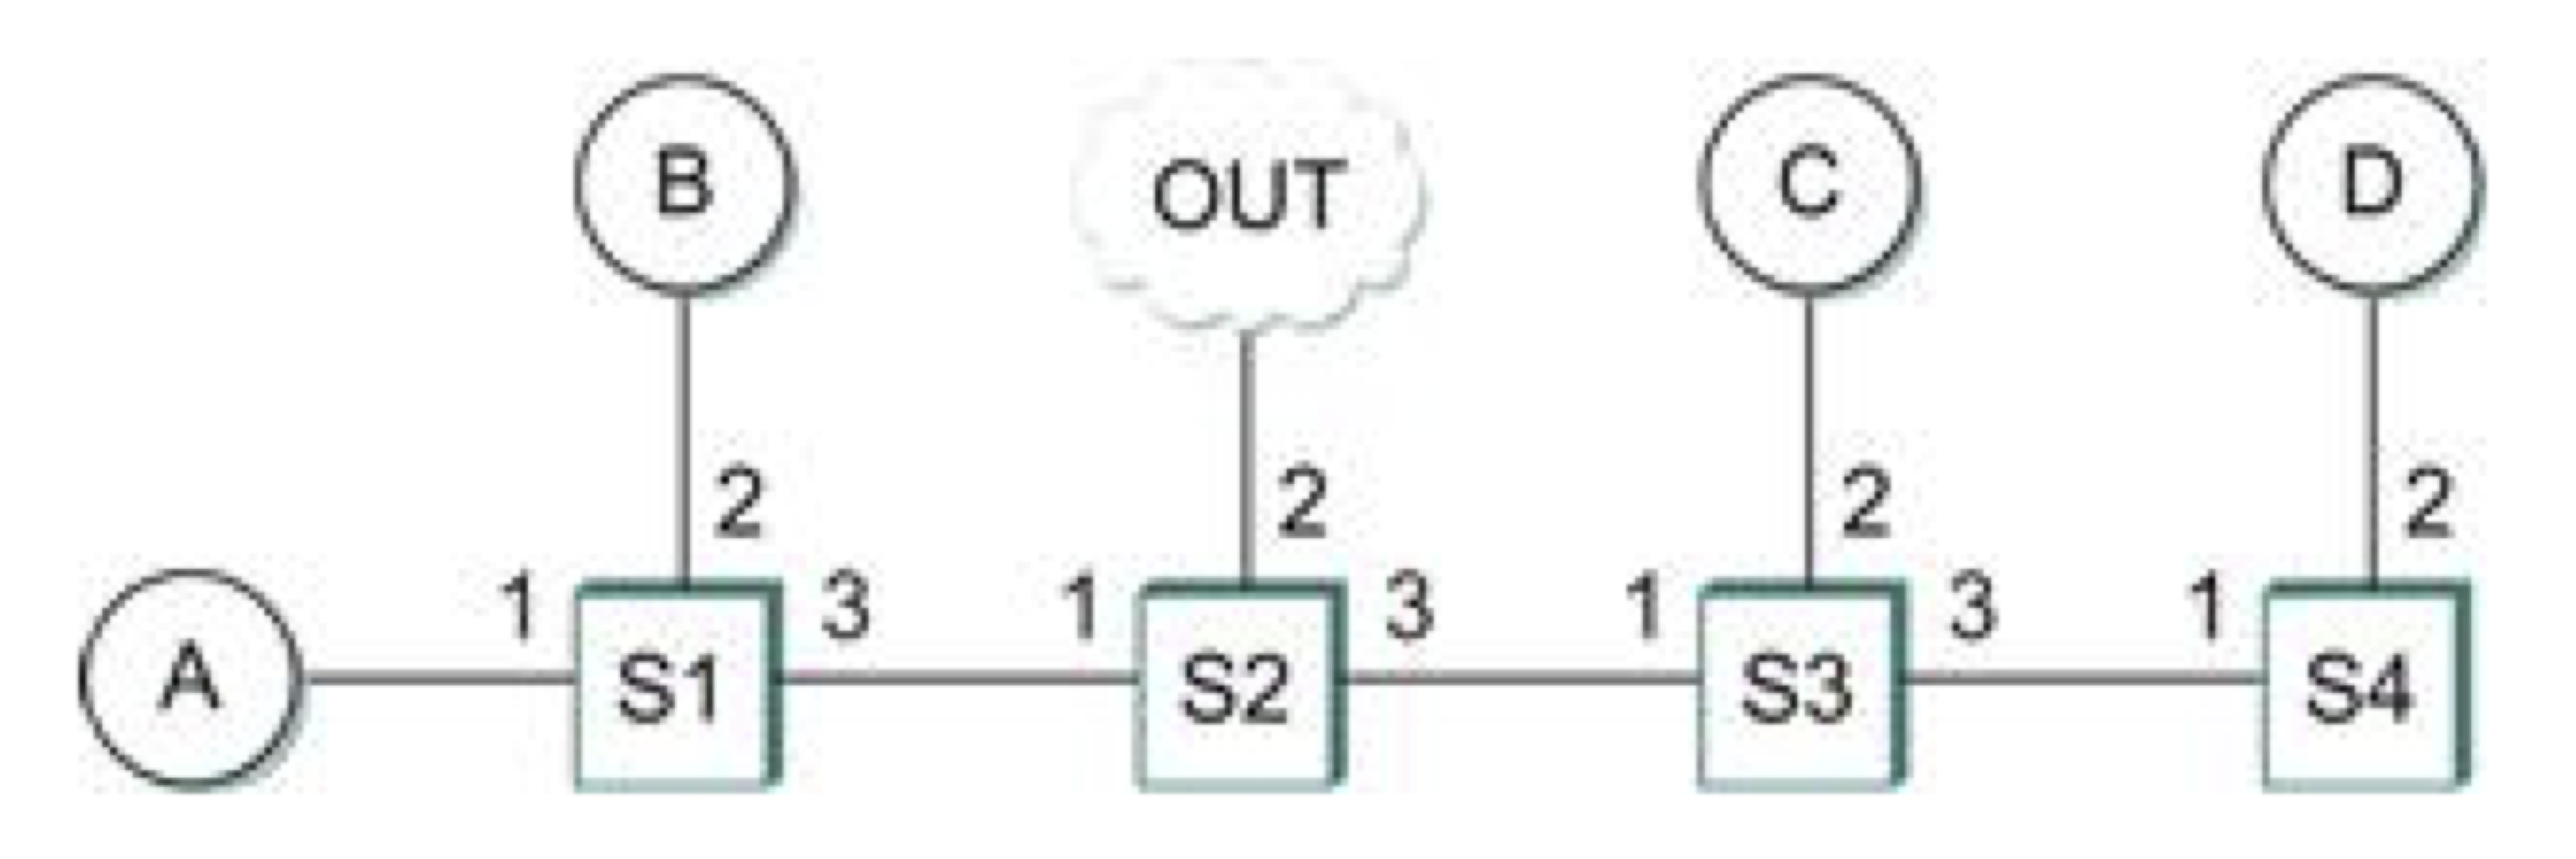
\includegraphics[width=0.6\linewidth]{fig/simple.png}
\end{center}
\begin{solution}
\end{solution}

\question[6] Create the forwarding table for switch 1 in the "fish" network below. How did you base your forwarding decisions?
\begin{center}
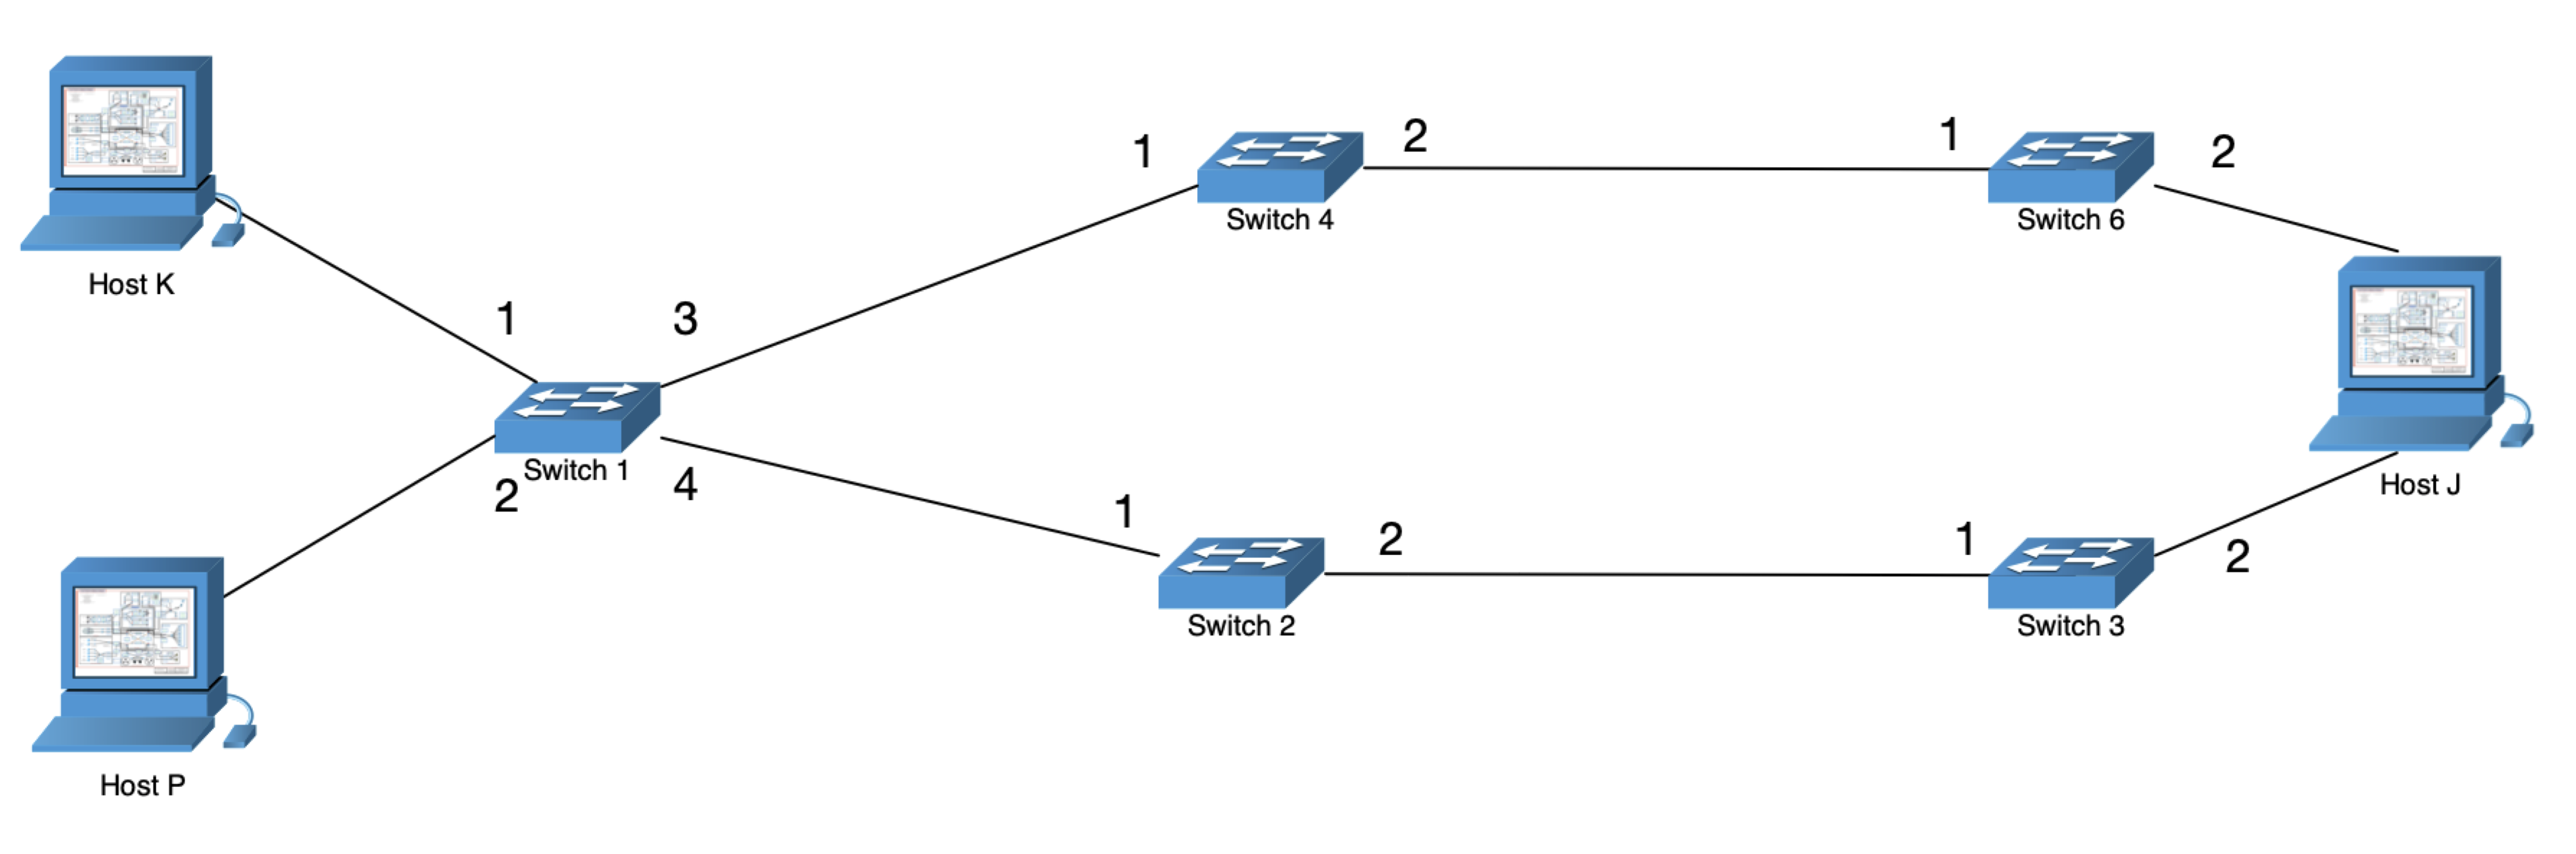
\includegraphics[width=1.0\linewidth]{fig/fish.png}
\end{center}
\begin{solution}
\end{solution}

\question[4] Some signaling errors can cause entire ranges of bits in a packet to be overwritten by all 0s or all 1s. Suppose all the bits in an IP packet, including the checksum are overwritten. Using what you know about the IPv4 packet header...
\begin{itemize}
\item Could a packet with all 0s be a legal IPv4 packet?
\item Could a packet with all 1s be a legal IPv4 packet?
\item Would the checksum catch either error?
\end{itemize}
Recall: the IPv4 checksum is the binary complement of the one's complement sum of all 16-bit words in the header.
\begin{solution}
\end{solution}

\question[8] Suppose a TCP message that contains 1024 bytes of data and the 20 byte TCP header is passed to IP for delivery across two networks interconnected by a router (i.e., it travesl from the source host to a router, and then from the router to the destination host). The first network has an MTU of 1024 bytes; the second has an MTU of 576 bytes. Give the sizes and offsets of each packet that arrives at the network layer of the destination host, keeping in mind that the network may have to fragment the packets. You should assume that all IP headers are 20 bytes.
\begin{solution}
\end{solution}

\question For the following network, give the global distance vector tables at each of the following time steps.
\begin{center}
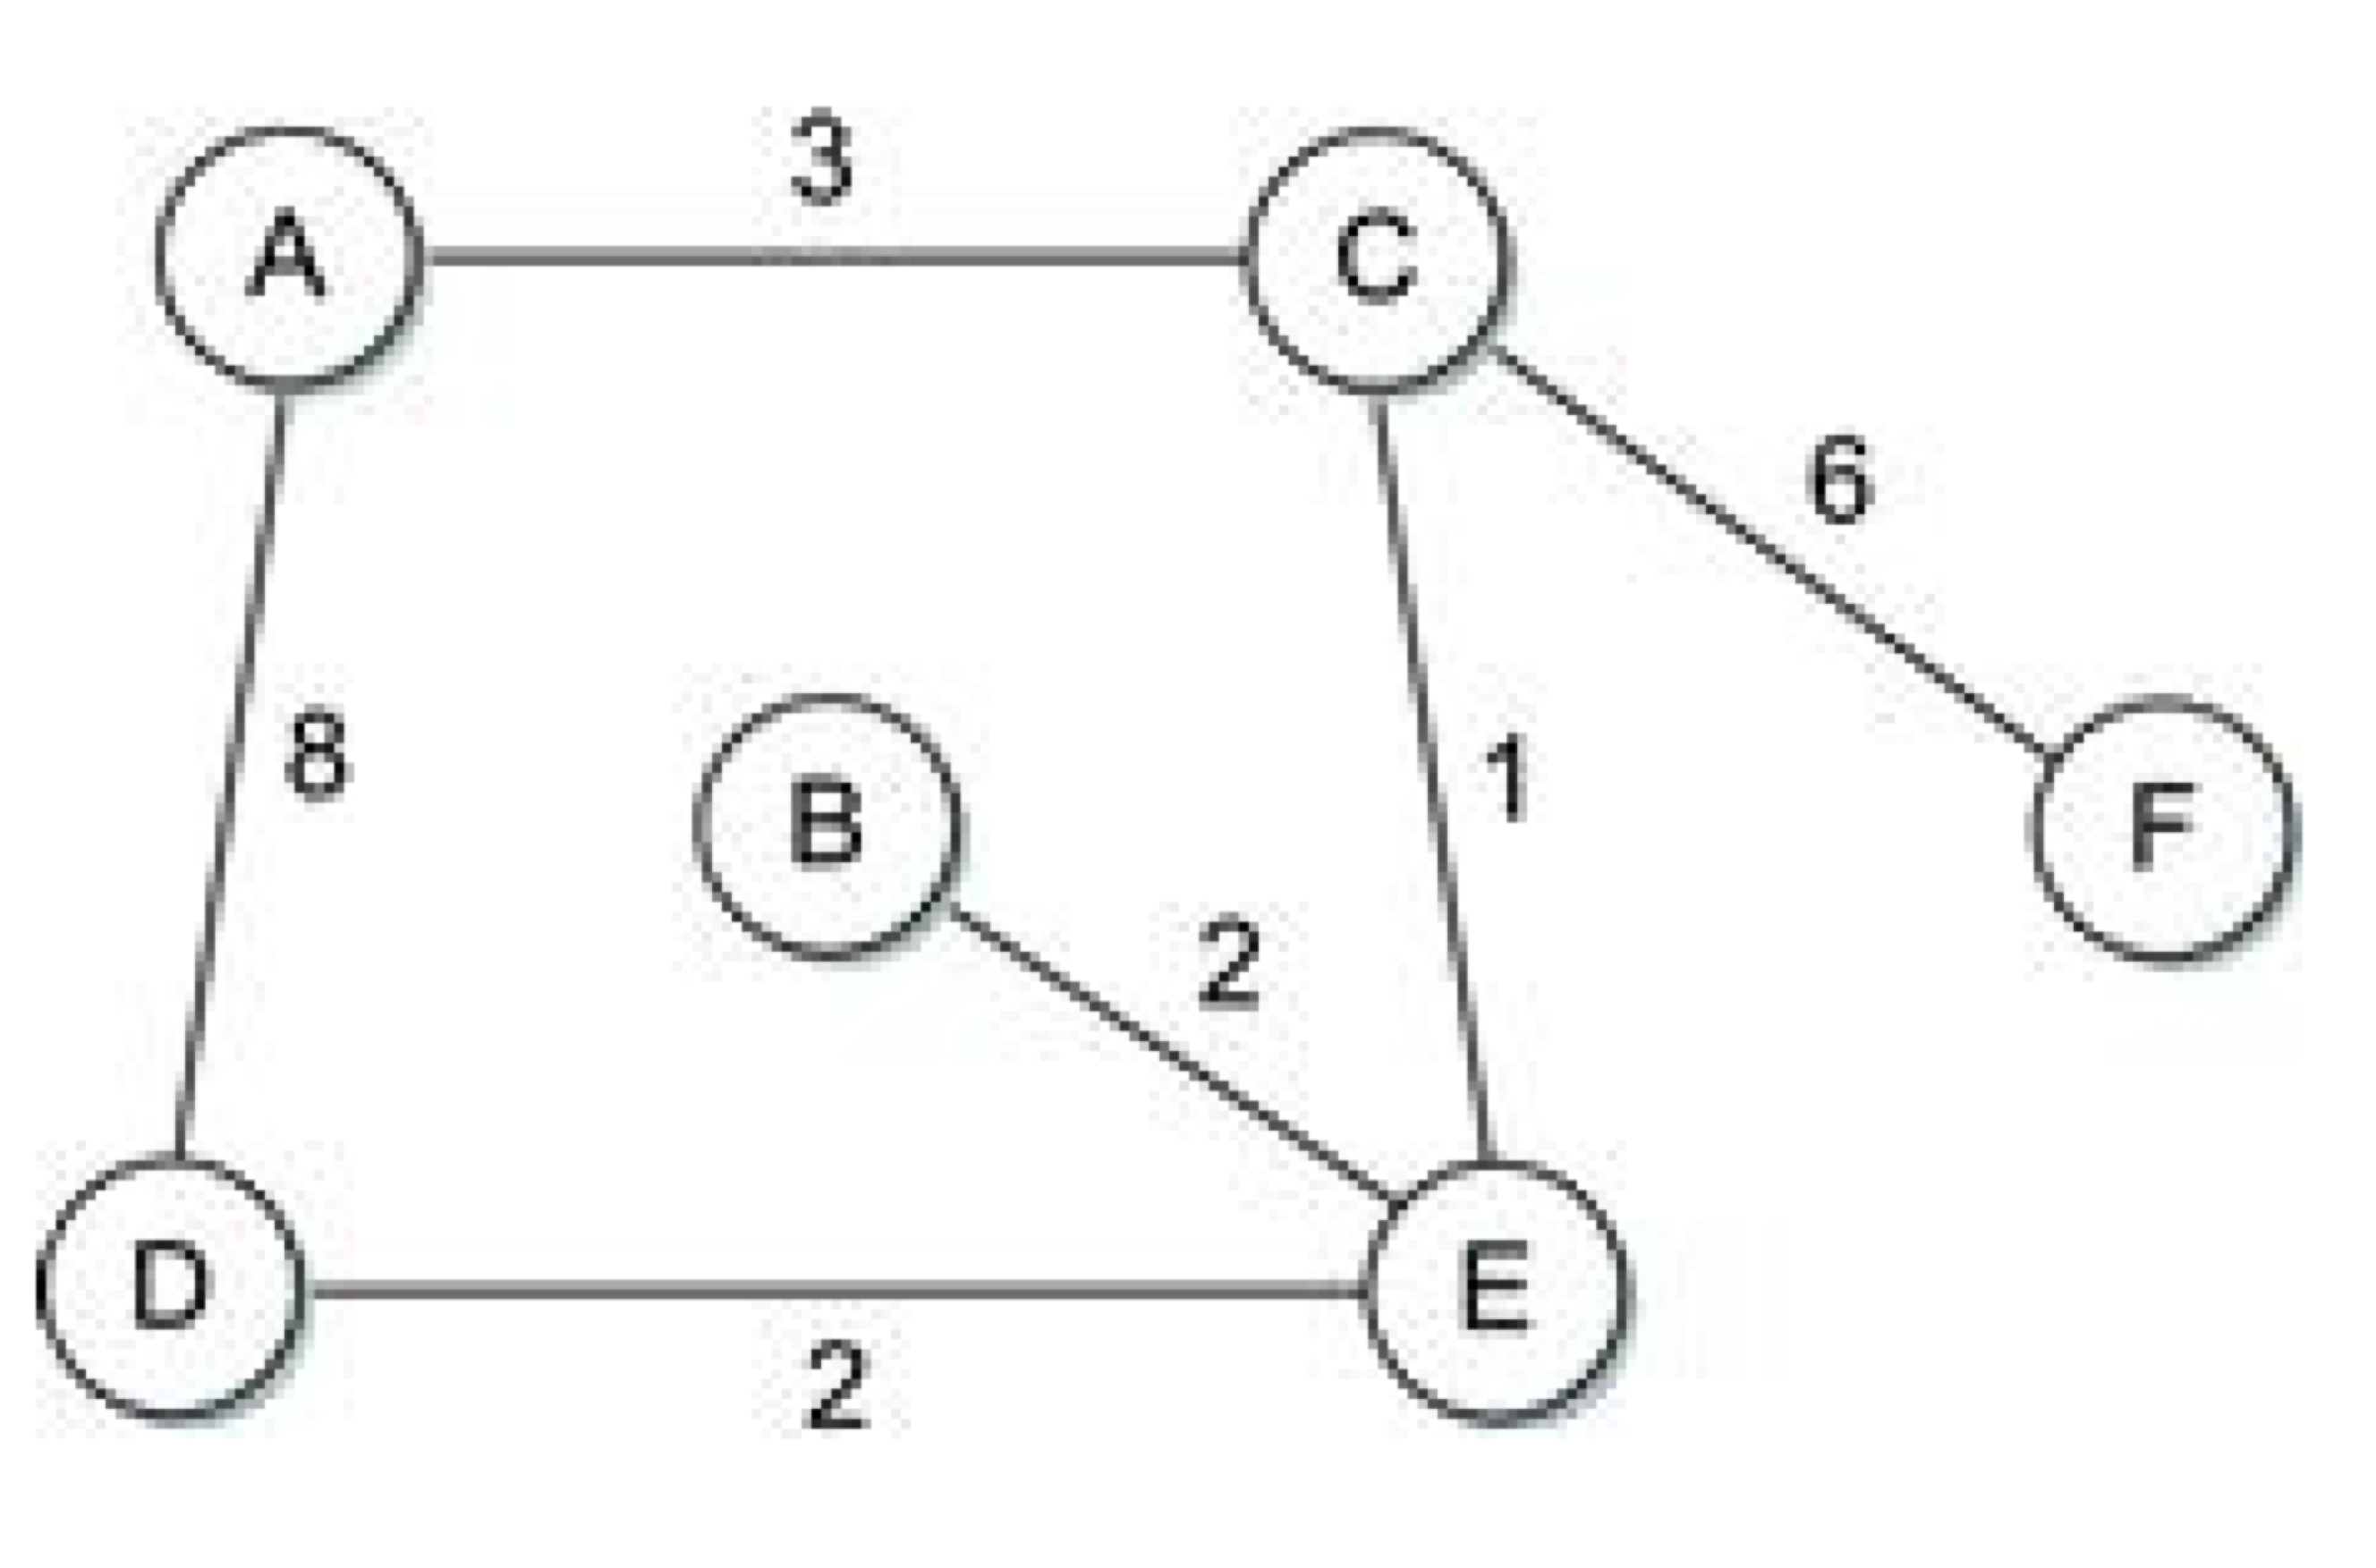
\includegraphics[width=0.4\linewidth]{fig/vector.png}
\end{center}
\begin{parts}
\part[4] Step 1: each node knows only the distances to its immediate neighbors.
\begin{solution}
\end{solution}
\part[6] Step 2: each node has reported its distance vector from part (a) to it's neighbors and updated.
\begin{solution}
\end{solution}
\part[6] Step 3: each node has reported its distance vector from part (b) to it's neighbors and updates.
\begin{solution}
\end{solution}
\end{parts}

\question Suppose the network from the previous problem has been upgraded to use Link State routing.
\begin{parts}
\part[4] Show the information sent out as part of the link state for each host.
\begin{solution}
\end{solution}
\part[10] Run the forward search algorithm (not Dijkstra's search) for node C. Make sure you check your final answer against the network to ensure you arrived at the correct forwarding decisions. You should assume that all of the link state packets have been flooded through the network.
\begin{solution}
\end{solution}
\end{parts}

\question[6] A particular organization is given the CIDR address range 210.81.112/20. What are all of the addresses owned by this organization? (List them as ranges, not individual values)
\begin{solution}
\end{solution}

\question A simple CIDR routing table is shown below. For each address, indicate which entry in the table it matches.
\begin{center}
\begin{tabularx}{0.3\linewidth}{>{\centering\arraybackslash}Xc}
\toprule
\emph{Address Mask} & \emph{Port} \\
\midrule
10.19.0.0/16 & 1 \\
10.19.128/17 & 2 \\
10.19.192/18 & 3 \\
10.19.192/19 & 4 \\
0.0.0.0/1    & 5 \\
1.0.0.0/1    & 6 \\
\bottomrule
\end{tabularx}
\end{center}
\begin{parts}
\part[2] 141.219.2.10
\part[2] 10.10.10.10
\part[2] 10.19.86.141
\part[2] 10.19.193.6
\part[2] 10.19.255.86
\part[2] 10.19.192.18
\end{parts}
\begin{solution}
\end{solution}

\question[8] Explain the software-defined networking approach to separating the routing and forwarding behavior. Why does it possibly lead to better routing decisions?
\begin{solution}
\end{solution}


\end{questions}
\end{document}
